\documentclass[10pt]{article}

\usepackage[a4paper,margin=1in]{geometry}
\usepackage[T1]{fontenc}
\usepackage[utf8]{inputenc}
\usepackage{lmodern}
\usepackage{microtype}
\usepackage{parskip}
\usepackage{amsmath,amssymb,amsthm,mathtools}
\usepackage{booktabs}
\usepackage{enumitem}
\usepackage{graphicx}
\usepackage{float}
\usepackage{xcolor}
\usepackage{algorithm}
\usepackage[noend]{algpseudocode}
\usepackage[numbers,sort&compress]{natbib}
\usepackage[hidelinks]{hyperref}
\usepackage[nameinlink,noabbrev]{cleveref}

\makeatletter
% Keep hyperref anchors for algorithmicx line numbers unique across
% multiple algorithms (cleveref refsteps ALG@line inside each one).
\providecommand{\theHALG@line}{\theALG@line}
\renewcommand{\theHALG@line}{\thealgorithm.\arabic{ALG@line}}
\makeatother

\newtheorem{theorem}{Theorem}[section]
\newtheorem{lemma}[theorem]{Lemma}
\newtheorem{corollary}[theorem]{Corollary}
\newtheorem{proposition}[theorem]{Proposition}
\newtheorem{observation}[theorem]{Observation}
\theoremstyle{definition}
\newtheorem{definition}[theorem]{Definition}
\newtheorem{remark}[theorem]{Remark}

\newcommand{\AC}{\mathsf{AC}}
\newcommand{\TC}{\mathsf{TC}}
\newcommand{\NC}{\mathsf{NC}}
\newcommand{\DLM}{\mathsf{DLM}}
\newcommand{\Pair}{\mathsf{Pair}}
\newcommand{\Path}{\mathsf{Path}}
\newcommand{\Unif}{\mathsf{Unif}}
\newcommand{\TV}{\mathrm{TV}}
\newcommand{\bits}{\{0,1\}}
\newcommand{\mask}{\mathtt{M}}
\newcommand{\ind}{\mathbf{1}}
\newcommand{\poly}{\operatorname{poly}}
\newcommand{\Stab}{\operatorname{Stab}}

\title{Sampling round complexity of diffusion language models in regular languages}
\author{Jiarui Zhang\\
Student ID: 2023010875\\
\texttt{jiarui-z23@mails.tsinghua.edu.cn}
\thanks{Mentor: Jingzhao Zhang at \texttt{jingzhaoz@mail.tsinghua.edu.cn}}}
\date{Summer Research Report, 2026}

\begin{document}
\maketitle

\begin{abstract}
Diffusion language models update many token positions in parallel.  We
study the number of rounds needed to generate the input--output pair
$(X,f_L(X))$, where $X$ is uniform and $f_L$ recognizes a fixed regular
language.

Our main technical result characterizes finite Markov chains whose complete
trajectories can be sampled from fair bits: this is possible for every horizon
exactly when all trajectory probabilities are dyadic.  Applying the result to
a DFA gives a randomized-$\AC^0$ sampler for every fixed binary regular
language.  As a corollary in the randomized-$\AC^0$ regime, two rounds suffice with
revision; without revision, a finite-monoid product tree gives
$O(\log n/\log\log n)$ rounds, with a matching lower bound for regular
languages outside $\AC^0$.  The results can be extended to the Transformer
regime under the equivalence between poly-width, finite-precision,
finite-depth transformers and $\AC^0$ circuits.
\end{abstract}

\section{Introduction}

Autoregressive language models expose an inherently sequential sampling
interface: the distribution of the next token is evaluated only after the
previous token has been fixed.  Diffusion language models (DLMs), by
contrast, repeatedly update many coordinates in parallel.  Their practical
appeal motivates a basic complexity question: how many parallel rounds are
needed to sample a prescribed distribution?

This question is meaningful only after restricting the computation performed
within a round.  Motivated by the connection between $\AC^0$ and
constant-precision Transformers established by Li et al.~\cite{li2024cot}, we
first work in the randomized-$\AC^0$ regime: each predictor is a
randomized-$\AC^0$ sampler, while the no-revision policy is an $\AC^0$
function.  A $D$-round sampler in this regime unrolls into a randomized
Boolean circuit of depth $O(D)$.  In \cref{sec:transformer}, we transfer the
lower and upper bounds to the specified Transformer regime.

Our target distributions are generated by fixed binary regular languages.
For $L\subseteq\bits^*$ and $f_L(x)=\ind[x\in L]$, let

\begin{equation}
  \Pair_{L,n}=(X,f_L(X)),\qquad X\sim\Unif(\bits^n).
  \label{eq:pair}
\end{equation}

The sampler must jointly produce a uniform input and its correct membership
bit.  Parity is the canonical example: recognition is outside $\AC^0$, whereas
its input--output pair distribution has a randomized-$\AC^0$ local sampler,
see \cref{alg:parity}; each output bit depends on at most two fair bits, so
the underlying process is even randomized-$\NC^0$.

\begin{algorithm}[ht]
\caption{Parity pair sampler in constant depth}
\label{alg:parity}
\begin{algorithmic}[1]
\State sample $u_1,\ldots,u_n\sim\Unif(\bits)$ independently
\State $X_1\gets u_1$
\For{$i=2,\ldots,n$}
  \State $X_i\gets u_{i-1}\oplus u_i$
\EndFor
\State $C\gets u_n\oplus1$ \Comment{$C=1$ iff $\bigoplus_i X_i=0$}
\State \Return $(X,C)$
\end{algorithmic}
\end{algorithm}

The second modeling decision is whether previously revealed tokens are
immutable.  A no-revision DLM only replaces masks by visible symbols.  A DLM
with revision may overwrite or remask visible coordinates, so the output
positions themselves provide reusable workspace.  Jiang et al.~\cite{jiang2026dlm}
formalize closely related parallel-sampling models and show that revision or
remasking can strictly increase their power.  We focus on fixed-length
generation with no extra chain-of-thought or padded coordinates.

\paragraph{Contributions.}
The report integrates two parts of the project into one self-contained chain
of results.

\begin{enumerate}[leftmargin=*,itemsep=2pt]
  \item Finite Markov-chain trajectories with dyadic probabilities admit
  randomized-$\AC^0$ samplers for every horizon; the dyadic condition is also
  necessary.
  \item Revision gives better round complexity than no-revision in both the
  randomized-$\AC^0$ and Transformer regimes: two rounds
  suffice with revision, while no-revision requires
  $\Theta(\log n/\log\log n)$ rounds for languages outside $\AC^0$ under the
  stated model.
\end{enumerate}

\section{Related Work}
\label{sec:related}

\paragraph{Transformers and circuit complexity.}
Formal Transformer models have been bounded or characterized using classical
circuit classes.  Under a constant-precision, constant-depth, polynomial-width
model, Li et al.~\cite{li2024cot} give the $\AC^0$ connection used here.
Other choices lead to different classes: saturated attention over
floating-point values, for example, admits a $\TC^0$ upper bound
\cite{merrill2022saturated}.  Svete et al.~\cite{svete2026reasoning} study
the reasoning power of diffusion language models and their relation to looped
and padded Transformer computation.

\paragraph{DLMs and parallel sampling.}
The theory of diffusion language models increasingly studies generation as a
sequence of parallel conditional updates.  Jiang et al.~\cite{jiang2026dlm}
connect DLM rounds to parallel sampling circuits, establish simulations with
chain-of-thought workspace, and show that revision or remasking enables
workspace reuse.  Our question is narrower: the output has exactly $n+1$
positions, sampling is exact, and each round is restricted to
randomized-$\AC^0$.

\paragraph{Complexity of distributions.}
The complexity of sampling a distribution can differ sharply from computing a
function that describes its support.  Viola developed a systematic circuit
view of distributions \cite{viola2012complexity}: parity and inner-product
pairs $(X,b(X))$ are generated \emph{exactly} by small randomized-$\AC^0$
circuits (for parity, each output bit depends on at most two fair bits, so
the underlying process is even randomized-$\NC^0$),
while for every symmetric function $b$ such as majority or $\mathrm{MOD}_3$,
randomized-$\AC^0$ circuits generate $(X,b(X))$ only approximately, up to an
exponentially small statistical distance.  Later work constructs an explicit
Boolean function $h$ such that small randomized-$\AC^0$ circuits cannot even
approximately sample $(U,h(U))$ to small statistical distance
\cite{viola2020sampling}.

\paragraph{Regular languages and shallow circuits.}
The algebraic theory of regular languages characterizes membership in
$\AC^0$ through aperiodicity of the stable syntactic monoid
\cite{barrington1992regular}.  Classical random-generation work constructs
logspace-uniform probabilistic circuits that generate words of
$L\cap\Sigma^n$ exactly uniformly in polylogarithmic depth, up to a bounded
rejection probability \cite{goldwurm2001random}.
These results provide useful neighboring generation models.  Our target
\cref{eq:pair} instead retains the uniform input word and appends its
membership label.

\paragraph{Random maps and Markov chains.}
A finite Markov chain can be represented by random maps, as in road-coloring
constructions \cite{yano2010road,jost2015random}; our overlap with this line
of work is only a coloring view.  Our objective is different: a
fixed linear number of fair bits, a constant-depth circuit, and the whole
trajectory at once.

\section{Models and Preliminaries}
\label{sec:model}

\subsection{Randomized constant-depth circuits}

$\AC^0$ is the class of Boolean functions computed by polynomial-size,
constant-depth circuits with unbounded-fan-in AND and OR gates and NOT gates.
A randomized-$\AC^0$ sampler is such a circuit whose inputs are independent
fair bits.  A family $C_n:\bits^{r(n)}\to\Omega_n$ samples a distribution
$\mathcal D_n$ exactly when

\begin{equation}
  \Pr[C_n(U_{r(n)})=z]=\Pr_{Z\sim\mathcal D_n}[Z=z]
  \quad\text{for every }z\in\Omega_n.
\end{equation}

Exactness immediately imposes an arithmetic constraint: every output atom of
a finite fair-bit sampler is dyadic, i.e., of the form $m/2^k$.

\subsection{DLM update rules}

Fix the vocabulary $V=\bits$ and a mask symbol $\mask$.  A sequence of length
$N$ begins at $\mask^N$.  In the no-revision model, a policy $F$ selects some
currently masked coordinates to unmask and a predictor $p$ supplies the
marginal distributions.  Given the current state, selected coordinates are
sampled independently:

\begin{algorithm}[ht]
\caption{No-revision DLM}
\label{alg:norevision}
\begin{algorithmic}[1]
\State $z\gets \mask^N$
\For{$t=1,\ldots,D$}
  \State $S\gets F(z)$, where $S\subseteq\{i:z_i=\mask\}$
  \ForAll{$i\in S$ \textbf{in parallel}}
    \State sample $z_i\sim p_i(\cdot\mid z)$ over $\bits$
  \EndFor
\EndFor
\State \Return $z$
\end{algorithmic}
\end{algorithm}

\begin{algorithm}[ht]
\caption{DLM with revision}
\label{alg:revision}
\begin{algorithmic}[1]
\State $z\gets \mask^N$
\For{$t=1,\ldots,D$}
  \ForAll{$i\in[N]$ \textbf{in parallel}}
    \State sample $z_i\sim p_i(\cdot\mid z)$ over $\bits\cup\{\mask\}$
  \EndFor
\EndFor
\State \Return $z$
\end{algorithmic}
\end{algorithm}

With revision, every coordinate may be updated to $0$, $1$, or $\mask$ in
every round.  A valid sampler for a binary target returns no mask with
probability one.  In both models, each local predictor is a
randomized-$\AC^0$ sampler: it receives the current state and fresh independent
fair bits and outputs one token.  The random bits used at different updated
coordinates are independent.  The no-revision policy $F$ is an $\AC^0$
circuit and has no random input.  In the Transformer realization, the
backbone computes the predictor's logits and the randomized local sampler is
obtained by independently decoding from them.

\subsection{Automata and aperiodicity}

For a DFA $\mathcal A=(Q,\Sigma,\delta,q_0,F)$, every word $u\in\Sigma^*$
induces a map on its states,

\begin{equation}
 T_u(q)=\delta^*(q,u).
\end{equation}

The set

\begin{equation}
 M_{\mathcal A}=\{T_u:u\in\Sigma^*\}
\end{equation}

is the transition monoid of $\mathcal A$, and
$\eta_{\mathcal A}:\Sigma^*\to M_{\mathcal A}$, defined by
$\eta_{\mathcal A}(u)=T_u$, is its transition morphism.

\begin{definition}[Stable monoid]
A positive integer $d$ is a \emph{stability index} of a morphism
$\eta:\Sigma^*\to M$ if

\begin{equation}
 \eta(\Sigma^d)=\eta(\Sigma^{2d}).
 \label{eq:stability-index}
\end{equation}

When stability indices exist, let $d_\eta$ be the smallest one.  The
\emph{stable monoid} of $\eta$ is

\begin{equation}
 \Stab(\eta)
 =\eta((\Sigma^{d_\eta})^*)
 =\{1\}\cup\eta(\Sigma^{d_\eta}).
 \label{eq:stable-monoid}
\end{equation}
\end{definition}

A stability index always exists when $M$ is finite.  Indeed, the sequence of
sets $\eta(\Sigma^j)$ is eventually periodic: for some $d_0,\ell\ge1$,
$\eta(\Sigma^{d_0})=\eta(\Sigma^{d_0+\ell})$.  Multiplication by
$\eta(\Sigma^k)$ gives the same equality after adding any $k\ge0$ to both
lengths.  Taking $d=\lceil d_0/\ell\rceil\ell$ therefore yields
$\eta(\Sigma^d)=\eta(\Sigma^{2d})$.  Thus $d_\eta$ is well-defined.
Applying \eqref{eq:stability-index} to $d_\eta$ also makes
$\eta(\Sigma^{d_\eta})$ closed under multiplication, which gives the second
equality in \eqref{eq:stable-monoid}.

A finite monoid is \emph{aperiodic} if every element $a$ satisfies
$a^{k+1}=a^k$ for some $k\ge1$.  Here and below, a nontrivial cycle means a
directed cycle of length at least $2$.

\begin{lemma}[Cycle criterion]
Let $g:H\to H$ be a self-map of a finite set.  Then $g^k=g^{k+1}$ for some
$k\ge1$ if and only if $g$ has no nontrivial cycle.  Consequently, a finite
transformation monoid is aperiodic if and only if none of its elements has a
nontrivial cycle.
\end{lemma}

\begin{proof}
If $g$ has a nontrivial cycle, then $g^m\ne g^{m+1}$ for every $m\ge1$.
Conversely, if every cycle of $g$ is a fixed point, then every orbit reaches a
fixed point within $|H|$ steps, so $g^{|H|}=g^{|H|+1}$.
\end{proof}

\begin{lemma}[$\AC^0$ recognition characterization]
\label{lem:stable-monoid-ac0}
Let $\mathcal A$ be the minimal DFA of a regular language $L$.  Then
$L\in\AC^0$ if and only if the stable monoid
$\Stab(\eta_{\mathcal A})$ is aperiodic.
\end{lemma}

This is the Barrington--Compton--Straubing--Th\'erien characterization
\cite{barrington1992regular}.  For a minimal DFA, the transition monoid is the
syntactic monoid, so $\Stab(\eta_{\mathcal A})$ is also called the stable
syntactic monoid of $L$.

\begin{lemma}[Aperiodic transition monoid implies $\AC^0$]
\label{lem:aperiodic-ac0}
If the full transition monoid $M_{\mathcal A}$ of a DFA is aperiodic, then the
language recognized by $\mathcal A$ is in $\AC^0$.
\end{lemma}

\begin{proof}
Minimize $\mathcal A$.  The transition monoid of the minimal DFA is a quotient
of $M_{\mathcal A}$.  A quotient of an aperiodic monoid is aperiodic, and
every submonoid is also aperiodic.  Thus the stable monoid of the minimal DFA
is aperiodic, and \cref{lem:stable-monoid-ac0} applies.  We use this implication
to compute all prefix states of an aperiodic block process in parallel.
\end{proof}

\begin{lemma}[Monotone DFA test]
\label{lem:monotone-ac0}
Suppose the states of a fixed DFA have a total order $\le$.  If every
character preserves this order, meaning that

\begin{equation}
 x\le y
 \quad\Longrightarrow\quad
 \delta(x,c)\le\delta(y,c)
\end{equation}

for all states $x,y$ and characters $c\in\Sigma$, then the language of the DFA
is in $\AC^0$.
\end{lemma}

\begin{proof}
Each character induces an order-preserving map, and a composition of such maps
is still order-preserving.  Therefore every word $w\in\Sigma^*$ induces an
order-preserving map $T_w$.

Fix a state $x$ and define $x_i=T_w^i(x)$.  Because the order is total, either
$x_1\le x_0$ or $x_1\ge x_0$.  In the first case, order preservation gives

\begin{equation}
 x_{i+1}=T_w(x_i)\le T_w(x_{i-1})=x_i,
\end{equation}

so the sequence keeps decreasing.  In the second case, the same argument shows
that it keeps increasing.  Since $Q$ is finite, the sequence must become
constant.  Thus, for every $x\in Q$, there is an integer $\ell_x$ such that

\begin{equation}
 T_w^{\ell_x}(x)=T_w^{\ell_x+1}(x).
\end{equation}

Let $N_w=\max_{x\in Q}\ell_x$.  Then

\begin{equation}
 T_w^{N_w}=T_w^{N_w+1}.
\end{equation}

$M_{\mathcal A}$ is aperiodic since $w$ was arbitrary, and
\cref{lem:aperiodic-ac0} applies.
\end{proof}

\section{Revision: Exact Sampling and Two Rounds}
\label{sec:revision}
\label{sec:markov}

Fix a finite Markov chain

\begin{equation}
 \mathcal M=(Q,\mu,P),
\end{equation}

where $\mu$ is the initial distribution on $Q$ and $P$ is the transition
matrix.

For a length $n$, a trajectory $\gamma=(x_0,\ldots,x_n)\in Q^{n+1}$ has
probability

\begin{equation}
 p_{\mathcal M}(\gamma)
 =\mu(x_0)\prod_{i=1}^{n}P(x_{i-1},x_i).
 \label{eq:pathprob}
\end{equation}

Write $\Path_n(\mathcal M)$ for the distribution on $Q^{n+1}$ defined by

\begin{equation}
 \Pr_{\gamma\sim\Path_n(\mathcal M)}
 \left[\gamma=(x_0,\ldots,x_n)\right]
 =p_{\mathcal M}(x_0,\ldots,x_n).
\end{equation}

Let $\mathbb D_{\ge0}$ be the set of nonnegative dyadic values.  Call
$\mathcal M$ \emph{transition-dyadic} when

\begin{equation}
 \mu(q),P(q,r)\in\mathbb D_{\ge0}
 \qquad\text{for all }q,r\in Q.
\end{equation}

Call $\mathcal M$ \emph{path-dyadic from $\mu$} when every trajectory atom is
dyadic:

\begin{equation}
 p_{\mathcal M}(\gamma)\in\mathbb D_{\ge0}
 \qquad\text{for every }n\ge0\text{ and }\gamma\in Q^{n+1}.
\end{equation}

Transition-dyadicity is sufficient but not necessary.  For example, on states
$\{a,b,c\}$, let

\begin{equation}
 \mu=\left(\frac34,\frac14,0\right),\qquad
 P=\begin{pmatrix}0&1/3&2/3\\0&1&0\\0&0&1\end{pmatrix}.
\end{equation}

The transitions $1/3$ and $2/3$ are not dyadic, but for every $n\ge1$ the only
positive trajectory atoms have probabilities

\begin{equation}
 \frac34\cdot\frac13=\frac14,\qquad
 \frac34\cdot\frac23=\frac12,\qquad
 \frac14.
\end{equation}

Thus the chain is path-dyadic.

\subsection{Transition-dyadic trajectories}

\begin{lemma}[Finite-state convergence]
\label{lem:finite-convergence}
Let $K$ be an irreducible and aperiodic transition matrix on a finite state
space.  Then $K$ has a unique stationary distribution $\pi$, with
$\pi(x)>0$ for every state $x$.  For every $\varepsilon>0$, there is
$m_\varepsilon$ such that, for every initial distribution $\lambda$ and every
$m\ge m_\varepsilon$,

\begin{equation}
 \left\|\lambda K^m-\pi\right\|_{\TV}<\varepsilon.
\end{equation}
\end{lemma}

See Levin and Peres, with contributions by Wilmer, \emph{Markov Chains and
Mixing Times}, Chapter 1 and Theorem 4.9.

\begin{proposition}[Ordered block-census sampling criterion]
\label{prop:ordered-block}
Let $\mathcal A=(Q,\bits,\delta,q_0,Q_{\mathrm{acc}})$ be a fixed binary DFA,
and let $L=L(\mathcal A)$.  Fix a block length $b\ge1$ and a total order

\begin{equation}
 Q=\{\xi_0<\xi_1<\cdots<\xi_{\ell-1}\}.
\end{equation}

Let $\Gamma=\bits^b$.  For $s,t\in Q$, define the block-transition census

\begin{equation}
 M_s(t)
 =
 \left|
  \left\{y\in\Gamma:\delta^*(s,y)=t\right\}
 \right|.
\end{equation}

For $\mathrm{Pfx}_k=\{\xi_0,\ldots,\xi_k\}$, set

\begin{equation}
 F_{s,\mathrm{Pfx}_k}
 =
 \sum_{t\in\mathrm{Pfx}_k}M_s(t).
\end{equation}

Assume that, for all $0\le i<\ell-1$ and $0\le k<\ell$,

\begin{equation}
 F_{\xi_i,\mathrm{Pfx}_k}
 \ge
 F_{\xi_{i+1},\mathrm{Pfx}_k}.
\end{equation}

Then there is a randomized-$\AC^0$ sampler for $\Pair_{L,n}$.
\end{proposition}

\begin{proof}
Let $N=2^b$ and set $F_{s,\mathrm{Pfx}_{-1}}=0$.  Order $\Gamma$
lexicographically.  We use the discrete common-quantile, or monotone,
coupling \cite[Chapter~1, Section~3]{thorisson2000coupling}: the same rank is
passed through the inverse cumulative census for every initial state.  For
$u\in\Gamma$, define $\tau_u(s)=\xi_k$ when

\begin{equation}
 F_{s,\mathrm{Pfx}_{k-1}}
 \le\operatorname{rank}(u)<
 F_{s,\mathrm{Pfx}_k}.
\end{equation}

Consider adjacent states $s=\xi_i<s'=\xi_{i+1}$.  If $\tau_u(s')=\xi_t$,
then

\begin{equation}
 \operatorname{rank}(u)
 <F_{s',\mathrm{Pfx}_t}
 \le F_{s,\mathrm{Pfx}_t}.
\end{equation}

Therefore $\tau_u(s)\le\xi_t=\tau_u(s')$.  Thus every $\tau_u$ preserves the
state order.

If $v=\xi_k$, then the two lists used in the rank matching below have the same
length:

\begin{equation}
 \left|\left\{u\in\Gamma:\tau_u(s)=v\right\}\right|
 =F_{s,\mathrm{Pfx}_k}-F_{s,\mathrm{Pfx}_{k-1}}
 =M_s(v)
 =\left|\left\{y\in\Gamma:\delta^*(s,y)=v\right\}\right|.
\end{equation}

Since the two sets have equal cardinality, we obtain block-cube permutations
$\pi_s:\Gamma\to\Gamma$ such that

\begin{equation}
 \delta^*(s,\pi_s(u))=\tau_u(s).
\end{equation}

Each $\pi_s$ is hard-coded into the circuit as a lookup table.

The sampler parses $z\in\bits^n$ as
$(u[1],\ldots,u[m],c)$ with $u[i]\in\Gamma$ and $c\in\bits^r$, where
$n=bm+r$.  It iterates $s[0]\gets q_0$,
$y[i]\gets\pi_{s[i-1]}(u[i])$, $s[i]\gets\tau_{u[i]}(s[i-1])$, and returns
$(y[1],\ldots,y[m],c)$ together with the label
$\ind[\delta^*(s[m],c)\in Q_{\mathrm{acc}}]$.

Every $\tau_u$ preserves the state order, so by \cref{lem:monotone-ac0} the
state reached after any block prefix is computable in $\AC^0$.  Compute all
these states in parallel; each output block is then a fixed lookup.  Thus the
sampling procedure is in randomized-$\AC^0$.
\end{proof}

\begin{theorem}[Transition-dyadic trajectories]
\label{thm:transition-dyadic}
Every transition-dyadic Markov chain has a randomized-$\AC^0$ sampler for
$\Path_n(\mathcal M)$.  It uses at most $v+sn$ fair bits, where $v$ depends on
$\mu$ and $s$ depends on $P$.
\end{theorem}

\begin{proof}
First consider only the directed support of $P$.  Let

\begin{equation}
 P_{\mathrm{bool}}(q,t)=\ind[P(q,t)>0],
\end{equation}

with powers taken over the Boolean semiring.  Since the Boolean powers
$P_{\mathrm{bool}}^j$ take only finitely many values, there are
$d_0,\ell\ge1$ with $P_{\mathrm{bool}}^{d_0}=P_{\mathrm{bool}}^{d_0+\ell}$;
take $a$ to be a multiple of $\ell$ with $a\ge d_0$.  Then

\begin{equation}
 P_{\mathrm{bool}}^a=P_{\mathrm{bool}}^{2a}.
\end{equation}

Set $P_{\mathrm{aperiodic}}:=P_{\mathrm{bool}}^a$; this Boolean matrix is
idempotent.

Now choose $s\ge1$ such that every $P(q,t)$ is an integer multiple of
$2^{-s}$, and set

\begin{equation}
 P_N=2^sP,
 \qquad
 \Gamma_s=\bits^s.
\end{equation}

Thus $P_N$ is an integer matrix whose rows sum to $2^s$.  For each $q$, assign
exactly $P_N(q,t)$ characters of $\Gamma_s$ to the transition $q\to t$.  This
defines

\begin{equation}
 \delta:Q\times\Gamma_s\longrightarrow Q.
\end{equation}

For a positive integer $c$, use blocks in
$\Gamma_s^{ac}\cong\bits^{sac}$.  For a block word
$w=w_1\cdots w_{ac}\in\Gamma_s^{ac}$, define

\begin{equation}
 \delta(q,w)
 =
 \delta(\cdots\delta(\delta(q,w_1),w_2)\cdots,w_{ac}).
\end{equation}

Then

\begin{equation}
 \left|
  \left\{w\in\Gamma_s^{ac}:\delta(q,w)=t\right\}
 \right|
 =
 P_N^{ac}(q,t)
 =
 2^{sac}P^{ac}(q,t).
\end{equation}

Its Boolean support is

\begin{equation}
 P_{\mathrm{bool}}^{ac}
 =
 P_{\mathrm{aperiodic}}^c
 =
 P_{\mathrm{aperiodic}},
\end{equation}

so its SCCs do not depend on $c$.

Let $R$ be a terminal SCC of $P_{\mathrm{aperiodic}}$.  Write
$R=\{t_1,\ldots,t_k\}$.  Split each state into two hidden copies, set

\begin{equation}
 H_R=\{t_1^-,\ldots,t_k^-,t_1^+,\ldots,t_k^+\},
\end{equation}

and order them as
$t_1^-<\cdots<t_k^-<t_1^+<\cdots<t_k^+$.  Let
$\phi(t_i^-)=\phi(t_i^+)=t_i$ and list the hidden copies as
$h_1<\cdots<h_{2k}$.  A block transfer of hidden states is encoded by a
nonnegative integer census

\begin{equation}
 N_{\mathrm{hidden},c}:H_R\times H_R\longrightarrow\mathbb Z_{\ge0}.
\end{equation}

It must first satisfy exact projection:

\begin{equation}
 \sum_{\substack{h'\in H_R\\\phi(h')=t}}
 N_{\mathrm{hidden},c}(h,h')
 =
 P_N^{ac}(\phi(h),t)
 \qquad(h\in H_R,\ t\in R).
\end{equation}

Summing over $t\in R$ gives a row sum of $2^{sac}$.

The key idea is to extend the order-preserving structure of
\cref{prop:ordered-block}, so we also require

\begin{equation}
 \sum_{\substack{\widetilde h\in H_R\\\widetilde h\le x}}
 N_{\mathrm{hidden},c}(h_j,\widetilde h)
 \ge
 \sum_{\substack{\widetilde h\in H_R\\\widetilde h\le x}}
 N_{\mathrm{hidden},c}(h_{j+1},\widetilde h)
\end{equation}

for every $1\le j<2k$ and $x\in H_R$.

Since $P_{\mathrm{aperiodic}}|_R$ is the all-one matrix,
\cref{lem:finite-convergence} applied to $P^a|_R$ gives a stationary
distribution $\pi_R$ and, for $1\le j\le2k$ and $1\le i\le k$,

\begin{equation}
 2^{-sac}P_N^{ac}(\phi(h_j),t_i)
 =
 P^{ac}(\phi(h_j),t_i)
 \longrightarrow
 \pi_R(t_i)
 \qquad(c\longrightarrow\infty).
\end{equation}

The construction is

\begin{equation}
 \begin{aligned}
  N_{\mathrm{hidden},c}(h_j,t_i^-)
  &=
  \left\lfloor
   \frac{2k+1-j}{2k+1}P_N^{ac}(\phi(h_j),t_i)
  \right\rfloor,\\
  N_{\mathrm{hidden},c}(h_j,t_i^+)
  &=
  \left\lceil
   \frac{j}{2k+1}P_N^{ac}(\phi(h_j),t_i)
  \right\rceil.
 \end{aligned}
\end{equation}

These formulas apply for $1\le j\le2k$ and $1\le i\le k$.  The two integers
sum exactly to $P_N^{ac}(\phi(h_j),t_i)$, so exact projection holds.

The rounding error in each integer count is at most $1$.  Therefore, for
$1\le j<2k$ and $1\le r\le k$,

\begin{equation}
 \begin{aligned}
  &2^{-sac}
  \sum_{i=1}^{r}
  \left(
   N_{\mathrm{hidden},c}(h_j,t_i^-)
   -
   N_{\mathrm{hidden},c}(h_{j+1},t_i^-)
  \right)\\
  &\qquad=
  \sum_{i=1}^{r}
  \left(
   \frac{2k+1-j}{2k+1}P^{ac}(\phi(h_j),t_i)
   -
   \frac{2k-j}{2k+1}P^{ac}(\phi(h_{j+1}),t_i)
  \right)
  +O(r2^{-sac})\\
  &\qquad\longrightarrow
  \frac{1}{2k+1}\sum_{i=1}^{r}\pi_R(t_i)>0.
 \end{aligned}
\end{equation}

For $1\le j<2k$ and $1\le r<k$, exact row sums similarly give

\begin{equation}
 \begin{aligned}
  &2^{-sac}
  \sum_{\substack{\widetilde h\in H_R\\\widetilde h\le t_r^+}}
  \left(
   N_{\mathrm{hidden},c}(h_j,\widetilde h)
   -
   N_{\mathrm{hidden},c}(h_{j+1},\widetilde h)
  \right)\\
  &\qquad=
  2^{-sac}
  \sum_{i=r+1}^{k}
  \left(
   N_{\mathrm{hidden},c}(h_{j+1},t_i^+)
   -
   N_{\mathrm{hidden},c}(h_j,t_i^+)
  \right)\\
  &\qquad=
  \sum_{i=r+1}^{k}
  \left(
   \frac{j+1}{2k+1}P^{ac}(\phi(h_{j+1}),t_i)
   -
   \frac{j}{2k+1}P^{ac}(\phi(h_j),t_i)
  \right)
  +O\left((k-r)2^{-sac}\right)\\
  &\qquad\longrightarrow
  \frac{1}{2k+1}\sum_{i=r+1}^{k}\pi_R(t_i)>0.
 \end{aligned}
\end{equation}

All prefix-sum differences are positive, and there are only finitely many
choices of $j$ and $r$.  Hence there is $c_R$ such that every ordered-cut
inequality holds for all $c\ge c_R$.  There are only finitely many terminal
SCCs, so one common $c\ge\max_R c_R$ works for all of them.

For $u\in\Gamma_s^{ac}$, let $\tau_u(h)$ be constructed as in
\cref{prop:ordered-block}, so $\tau_u$ is order-preserving on each split
terminal SCC.  Consequently, every composition of these maps is also
order-preserving there and has no nontrivial cycle.

For $h$ in a terminal SCC and $t\in Q$, the sets

\begin{equation}
 D_{h,t}
 =
 \left\{
  u\in\Gamma_s^{ac}:\phi(\tau_u(h))=t
 \right\}
\end{equation}

and

\begin{equation}
 W_{h,t}
 =
 \left\{
  w\in\Gamma_s^{ac}:\delta(\phi(h),w)=t
 \right\}
\end{equation}

have the same cardinality.  Match them for every $t$.  The union of these
matches is a block-cube permutation

\begin{equation}
 \pi_h:\Gamma_s^{ac}\longrightarrow\Gamma_s^{ac}
\end{equation}

such that

\begin{equation}
 \delta(\phi(h),\pi_h(u))=\phi(\tau_u(h)).
 \label{eq:projection-block}
\end{equation}

We now rule out nontrivial cycles using the cycle criterion.  Every hidden
transition used above projects to an edge of $P_{\mathrm{aperiodic}}$.  The
condensation graph of $P_{\mathrm{aperiodic}}$ is acyclic, so every map stays
in its current SCC or moves downstream.  Therefore any nontrivial cycle of a
composition of seed maps must lie entirely in one SCC.

It remains to prevent such nontrivial cycles inside transient SCCs.  Let $C$
be a transient SCC and keep only one hidden copy $h_q$ of each $q\in C$, with
$\phi(h_q)=q$.  Since $C$ is transient for $P^a$,

\begin{equation}
 \sum_{q\in C}P^{ac}(q,C)\longrightarrow0.
\end{equation}

Increase $c$ further, if necessary, so that the terminal CDF order still holds
and

\begin{equation}
 \sum_{q\in C}P^{ac}(q,C)<1
\end{equation}

for every transient SCC $C$.  Equivalently,

\begin{equation}
 \sum_{q\in C}\sum_{t\in C}P_N^{ac}(q,t)<2^{sac}.
\end{equation}

This allows us to assign a different seed to every internal transition
$h_q\to h_t$, with $q,t\in C$.  Thus each seed induces at most one transition
inside $C$, and any composition does as well.  The corresponding block-cube
permutations are constructed in the same way.

By the cycle criterion, the seed-generated monoid is aperiodic.

Choose $v\ge0$ such that every $\mu(q)$ is an integer multiple of $2^{-v}$,
and fix a lookup $g:\bits^v\to Q$ whose output has law $\mu$.  Also fix one
hidden copy $\iota(q)\in\phi^{-1}(q)$ for every $q$.  The complete sampler is
\cref{alg:samplepath}.

\begin{algorithm}[ht]
\caption{SamplePath: sampling a transition-dyadic trajectory}
\label{alg:samplepath}
\begin{algorithmic}[1]
\State \textbf{Input:} $st\in\bits^v$ and $z\in\bits^{sn}$
\State write $n=ac\cdot m+r$ with $0\le r<ac$
\State parse $z$ as $(u[1],\ldots,u[m],e[1],\ldots,e[r])$, with
  $u[i]\in\Gamma_s^{ac}$ and $e[j]\in\Gamma_s$
\State $x[0]\gets g(st)$ \Comment{sample the initial visible state from $\mu$}
\State $h[0]\gets\iota(x[0])$ \Comment{choose its fixed hidden copy}
\For{$i=1,\ldots,m$}
  \State $y[i]\gets\pi_{h[i-1]}(u[i])$
  \State $h[i]\gets\tau_{u[i]}(h[i-1])$
  \State parse $y[i]$ as $(y[i,1],\ldots,y[i,ac])$
  \For{$j=1,\ldots,ac$}
    \State $x[(i-1)ac+j]\gets\delta(x[(i-1)ac+j-1],y[i,j])$
  \EndFor
\EndFor
\For{$j=1,\ldots,r$}
  \State $x[mac+j]\gets\delta(x[mac+j-1],e[j])$
\EndFor
\State \Return $(x[0],\ldots,x[n])$
\end{algorithmic}
\end{algorithm}

By \cref{lem:aperiodic-ac0}, the hidden state reached after any block prefix
is computable in $\AC^0$.  Compute all block-prefix states in parallel; the
transformed blocks, their constant-length internal paths, and the final
remainder are fixed lookups.  Thus the sampler is randomized-$\AC^0$.
\end{proof}

\subsection{A finite dyadic lift}

Path-dyadic chains reduce to the preceding theorem by splitting states into
finite fibers.

\begin{theorem}[Dyadic projection]
\label{thm:projection}
Every fixed path-dyadic Markov chain is the coordinatewise projection of a
fixed transition-dyadic Markov chain.  More precisely, there are a finite
chain $\widetilde{\mathcal M}=(\widetilde Q,\widetilde\mu,\widetilde P)$ and
a map $\phi:\widetilde Q\to Q$ with the following property.  If
$(\widetilde X_i)_{i\ge0}$ is the Markov chain with initial distribution
$\widetilde\mu$ and transition matrix $\widetilde P$, then, for every $n\ge0$
and every $(x_0,\ldots,x_n)\in Q^{n+1}$,

\begin{equation}
 \Pr[\phi(\widetilde X_0)=x_0,\ldots,
      \phi(\widetilde X_n)=x_n]
 =p_{\mathcal M}(x_0,\ldots,x_n)
 =\mu(x_0)\prod_{i=1}^{n}P(x_{i-1},x_i).
\end{equation}
\end{theorem}

\begin{proof}
Assume every state is reachable with positive probability from $\mu$.
Otherwise, discard the unreachable states; this does not change the
trajectory law.

We first construct positive integer weights $(w_q)_{q\in Q}$ satisfying

\begin{equation}
 \frac{\mu(q)}{w_q}\in\mathbb D_{\ge0},\qquad
 \frac{w_qP(q,r)}{w_r}\in\mathbb D_{\ge0}.
 \label{eq:weightcondition}
\end{equation}

Indeed, a positive edge satisfies
$P(q,r)=p_{\mathcal M}(\gamma r)/p_{\mathcal M}(\gamma)$ for any positive
trajectory $\gamma$ ending at $q$, so every positive transition is rational.

Fix an odd prime $p$.  For a positive rational $a/b$ in lowest terms, define
$v_p(a/b)$ as the exponent of $p$ in $a$ minus its exponent in $b$.  Let

\begin{equation}
 \Gamma(r)
 =
 \left\{
  \gamma=(x_0,\ldots,x_n):
  n\ge0,\ x_n=r,\ p_{\mathcal M}(\gamma)>0
 \right\}
\end{equation}

be the set of positive-probability finite trajectories ending at $r$, and
define

\begin{equation}
 0\le\alpha_r^p
 =
 \min_{\gamma\in\Gamma(r)}
 v_p\!\left(p_{\mathcal M}(\gamma)\right).
\end{equation}

Equivalently, add a source $*$ with an edge $*\to q$ of weight
$v_p(\mu(q))$ whenever $\mu(q)>0$, and give each positive edge $q\to r$
weight $v_p(P(q,r))$.  Then $\alpha_r^p$ is the shortest-path distance from
$*$ to $r$.  Path-dyadicity rules out negative cycles and makes this distance
nonnegative, so the minimum is attained.

If $P(q,r)>0$, append the edge $q\to r$ to a trajectory attaining
$\alpha_q^p$.  This gives

\begin{equation}
 \alpha_r^p\le\alpha_q^p+v_p(P(q,r)).
\end{equation}

If $\mu(r)>0$, the length-zero trajectory $(r)$ similarly gives

\begin{equation}
 \alpha_r^p\le v_p(\mu(r)).
\end{equation}

Now set

\begin{equation}
 w_r
 =
 \prod_{p\text{ odd prime}}p^{\alpha_r^p}.
\end{equation}

This product is finite because the finitely many nonzero entries of $\mu$ and
$P$ involve only finitely many odd primes.

For every odd prime $p$, the two preceding inequalities give

\begin{equation}
 v_p\!\left(\frac{\mu(r)}{w_r}\right)
 =
 v_p(\mu(r))-\alpha_r^p
 \ge0
\end{equation}

when $\mu(r)>0$, and

\begin{equation}
 v_p\!\left(\frac{w_qP(q,r)}{w_r}\right)
 =
 \alpha_q^p+v_p(P(q,r))-\alpha_r^p
 \ge0
\end{equation}

when $P(q,r)>0$.  A positive rational is dyadic exactly when its valuation at
every odd prime is nonnegative; zero entries are dyadic as well.  Thus the
weights satisfy \cref{eq:weightcondition}.

Split state $q$ into the fiber
$F_q=\{(q,1),\ldots,(q,w_q)\}$ and let
$\widetilde Q=\bigsqcup_qF_q$.  Choose $s$ so that

\begin{equation}
 m_{q,r}
 =
 2^s\frac{w_qP(q,r)}{w_r}
\end{equation}

is an integer for every $q,r$.  For each $q$, choose an integer matrix
$C^{(q)}$ with rows indexed by $F_q$ and columns by $\widetilde Q$, such that
every row sums to $2^s$ and every column in $F_r$ sums to $m_{q,r}$.  Such a
matrix exists because both total sums equal $2^sw_q$.

For $h\in F_q$, define

\begin{equation}
 \widetilde\mu(h)=\frac{\mu(q)}{w_q}\quad(h\in F_q),
 \qquad
 \widetilde P(h,h')=\frac{C^{(q)}(h,h')}{2^s}.
 \label{eq:lift}
\end{equation}

Both are dyadic.  We prove by induction on $n$ that, for every positive
trajectory $\gamma=(x_0,\ldots,x_n)$ and every $h\in F_{x_n}$,

\begin{equation}
 \Pr[\phi(\widetilde X_0)=x_0,\ldots,
      \phi(\widetilde X_{n-1})=x_{n-1},\widetilde X_n=h]
 =\frac{p_{\mathcal M}(\gamma)}{w_{x_n}}.
\end{equation}

For $n=0$, this is the definition of $\widetilde\mu$.  Suppose it holds for a
trajectory $\gamma$ ending at $q$.  For every positive extension $\gamma r$
and every $h'\in F_r$, the column-sum condition on $C^{(q)}$ gives

\begin{align}
 \sum_{h\in F_q}\frac{p_{\mathcal M}(\gamma)}{w_q}
       \widetilde P(h,h')
 &=
  \frac{p_{\mathcal M}(\gamma)}{w_q}
  \sum_{h\in F_q}\frac{C^{(q)}(h,h')}{2^s}\\
 &=\frac{p_{\mathcal M}(\gamma)}{w_q}
   \frac{m_{q,r}}{2^s}\\
 &=\frac{p_{\mathcal M}(\gamma)P(q,r)}{w_r}
 =\frac{p_{\mathcal M}(\gamma r)}{w_r}.
\end{align}

This proves the induction step.  Summing over $h\in F_{x_n}$ gives
$p_{\mathcal M}(\gamma)$, proving the projection claim.
\end{proof}

\begin{corollary}[Exact sampling characterization]
\label{cor:characterization}
A fixed finite Markov chain has a randomized-$\AC^0$ trajectory sampler for
all horizons if and only if it is path-dyadic.
\end{corollary}

\begin{proof}
A sampler using $r_n$ fair bits assigns every atom an integer multiple of
$2^{-r_n}$, proving necessity.  For sufficiency, apply
\cref{thm:projection} followed by \cref{thm:transition-dyadic} and project each
hidden output coordinate through the fixed map $\phi$.
\end{proof}

\subsection{From Markov Trajectories to Regular-Language Pairs}
\label{sec:regular}

The preceding characterization applies directly to a DFA driven by a uniform
random input.

\begin{corollary}[Binary regular-language sampling]
\label{cor:regular}
Every fixed binary regular language $L\subseteq\bits^*$ has a
randomized-$\AC^0$ sampler for $\Pair_{L,n}$.
\end{corollary}

\begin{proof}
Fix a DFA $\mathcal A=(Q,\bits,\delta,q_0,F)$ for $L$ and define

\begin{equation}
 A(q,r)=\{a\in\bits:\delta(q,a)=r\},\qquad
 P(q,r)=\frac{|A(q,r)|}{2}.
 \label{eq:dfa-chain}
\end{equation}

Thus

\begin{equation}
 P(q,r)\in\left\{0,\frac12,1\right\}
 \subseteq\mathbb D_{\ge0}.
\end{equation}

Hence the chain is transition-dyadic and therefore path-dyadic.

With $\mu=e_{q_0}$, \cref{cor:characterization} samples its state trajectory

\begin{equation}
 (Y_0,Y_1,\ldots,Y_n),\qquad Y_0=q_0.
\end{equation}

Conditioned on this path, independently sample $X_{i+1}$ by

\begin{equation}
 \Pr[X_{i+1}=a\mid Y_i,Y_{i+1}]
 =\frac{\ind[\delta(Y_i,a)=Y_{i+1}]}
 {\sum_{b\in\bits}\ind[\delta(Y_i,b)=Y_{i+1}]}
 \in\{0,1/2,1\}.
 \label{eq:posterior-letter}
\end{equation}

for $0\le i<n$ and $a\in\bits$.  Each coordinate uses at most one fresh fair
bit.  Then $X=(X_1,\ldots,X_n)\sim U_n$ and

\begin{equation}
 C=\ind[Y_n\in F]=f_L(X).
\end{equation}

Thus $(X,C)$ has distribution $\Pair_{L,n}$, and the postprocessing is in
randomized-$\AC^0$.
\end{proof}

\begin{remark}[Why a sequential DFA becomes shallow]
The direct recurrence $Y_{i+1}=\delta(Y_i,X_{i+1})$ is sequential.  The
sampler does not evaluate this recurrence on the original fair bits.  It first
applies a measure-preserving cube reparameterization whose induced block
transformations generate an aperiodic monoid.  Aperiodicity is the bridge that
makes every prefix state simultaneously computable in $\AC^0$.
\end{remark}

\subsection{Two Rounds with Revision}
\label{sec:dlm}

The randomized circuit from \cref{cor:regular} can be embedded into two DLM
rounds without adding output positions.

\begin{theorem}[Two-round revision sampling]
\label{thm:two-round}
For every fixed binary regular language $L$ and every $n\ge1$, a
randomized-$\AC^0$ DLM with revision samples $\Pair_{L,n}$ in at most two
rounds.
\end{theorem}

\begin{proof}
Fix a DFA $\mathcal A=(Q,\bits,\delta,q_0,F_{\mathcal A})$ for $L$.  The
construction in \cref{cor:regular} uses at most $n$ fair bits for the DFA
trajectory.  In round one, sample the first $n$ coordinates independently and
uniformly, and set the label coordinate to a fixed placeholder.  In round two,
map the first-round bits to the state trajectory $(Y_0,\ldots,Y_n)$ and update
each input coordinate according to \cref{eq:posterior-letter}.  These updates
are coordinatewise once the trajectory is fixed.  Set the label to
$\ind[Y_n\in F_{\mathcal A}]$.  The output law is $\Pair_{L,n}$.
\end{proof}

For parity, one round is impossible: a one-round update from a fully masked
state is a product distribution, whereas uniform odd parity on $n+1$ bits is
not a product distribution.  Hence the revision complexity of parity is
exactly two.

\section{No-Revision Round Complexity}
\label{sec:no-revision}

Revision destroys the irreversible trace structure used in lower bounds.  In
the no-revision model, however, every completed output fixes the symbols that
must have appeared whenever a position was first exposed.

For comparison, the fully sequential autoregressive regime inside
randomized-$\AC^0$ already has a clean characterization.

\begin{observation}[Autoregressive sampling]
In the randomized-$\AC^0$ autoregressive regime, the family
$\{\Pair_{L,n}\}_{n\ge1}$ is sampleable if and only if $L\in\AC^0$.
\end{observation}

\begin{proof}
If $L\in\AC^0$, sample the input bits independently and uniformly, then
output $f_L(x)$.  Conversely, an exact autoregressive sampler must output
$f_L(x)$ after the full input $x$ is visible.  The final predictor is therefore
supported on a single bit for every $x$; fixing its random input gives an
$\AC^0$ circuit that computes $f_L$.
\end{proof}

The mask profile itself can carry a constant-size monoid summary while the
ordinary output coordinates remain the only available workspace:

\begin{figure}[H]
 \centering
 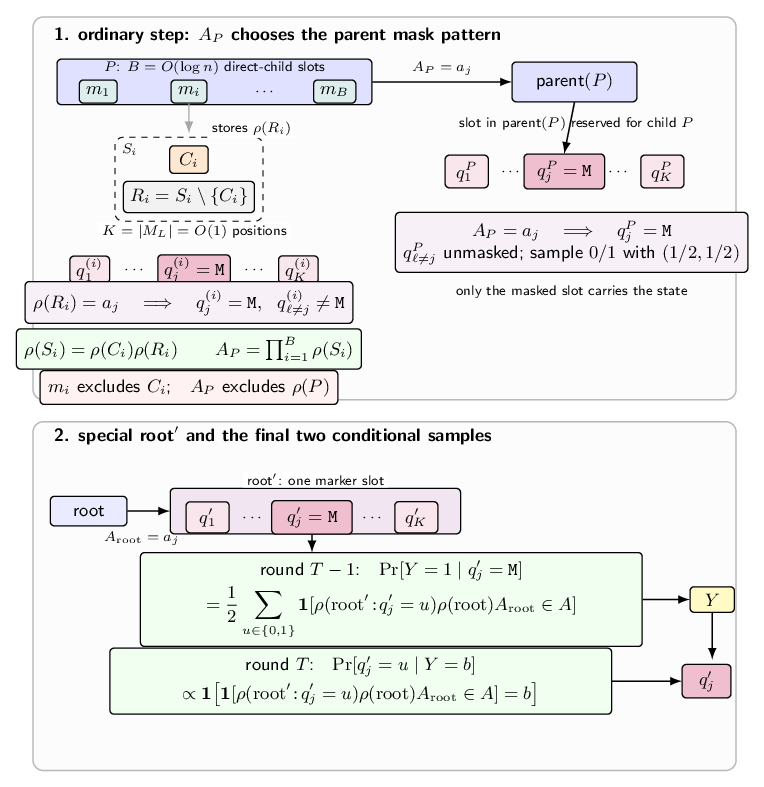
\includegraphics[width=0.96\linewidth]{../blog/regular-language-segments.png}
 \caption{No-revision product-tree summaries stored in the mask profile of
 ordinary output coordinates.}
 \label{fig:segments}
\end{figure}

\begin{theorem}[No-revision bounds]
\label{thm:no-revision}
In the randomized-$\AC^0$ no-revision model, every fixed binary regular
language has an $O(\log n/\log\log n)$-round sampler for $\Pair_{L,n}$.  Under
the exact finite-fair-bit local-kernel model above, if $L\notin\AC^0$, then
every such sampler requires $\Omega(\log n/\log\log n)$ rounds.
\end{theorem}

\subsection{Upper bound: a high-arity monoid tree}

Use the standard finite-monoid product tree for regular languages.  Lay the
tree out in depth-first index order, so that each subtree occupies a
contiguous coordinate interval, including the internal positions assigned to
its root.  Fix a finite monoid $M_L$, a morphism
$\rho:\bits^*\to M_L$, and an accepting set $F_{\mathrm{acc}}\subseteq M_L$
such that

\begin{equation}
 f_L(x)=\ind[\rho(x)\in F_{\mathrm{acc}}].
\end{equation}

Equivalently, $\rho(w)$ records the DFA transition induced by a substring
$w$; applied to the start state, it gives the DFA state after reading $w$.

Enumerate

\begin{equation}
 M_L=\{a_1,\ldots,a_K\},\qquad K=|M_L|=O(1),
\end{equation}

and take a branching factor $B=\Theta(\log n)$.  The sampler uses a $B$-ary
product tree over the first $n$ output coordinates.  A marker slot is not an
extra alphabet symbol: it is a constant-size block of ordinary output
coordinates whose mask pattern carries a monoid value.  In the convention
used below, one coordinate in the slot is masked, and the index of that
masked coordinate encodes the value.

At an ordinary node $P$, write its direct-child subtrees in string order as
$S_1,\ldots,S_B$.  For each child subtree $S_i$, let $C_i$ be the root
coordinate of that subtree and let

\begin{equation}
 R_i=S_i\setminus\{C_i\}.
\end{equation}

The slot $m_i$ reserved for child $S_i$ consists of $K$ positions
$q^{(i)}_1,\ldots,q^{(i)}_K$.  It stores only the remainder value
$\rho(R_i)$, not the root coordinate $C_i$, by the one-mask convention

\begin{equation}
 \rho(R_i)=a_j
 \quad\Longleftrightarrow\quad
 q^{(i)}_j=\mask,\qquad q^{(i)}_{\ell\ne j}\ne\mask.
\end{equation}

When this child slot is consumed, the slot's still-masked coordinate is also
unmasked and sampled as a fair bit.  After the coordinate $C_i$ is sampled,
the predictor can compute

\begin{equation}
 \rho(S_i)=\rho(C_i)\rho(R_i).
\end{equation}

The value passed from $P$ to $\mathrm{parent}(P)$ is then

\begin{equation}
 A_P=\prod_{i=1}^{B}\rho(S_i).
\end{equation}

As in \cref{fig:segments}, $A_P$ still excludes $\rho(P)$ itself.  If
$A_P=a_j$, then in the slot of $\mathrm{parent}(P)$ reserved for child $P$,
the next round creates the mask pattern

\begin{equation}
 q^{\mathrm{parent}(P)}_j=\mask,\qquad
 q^{\mathrm{parent}(P)}_{\ell\ne j}\ne\mask,
\end{equation}

sampling every newly unmasked
$q^{\mathrm{parent}(P)}_{\ell\ne j}$ as a fair bit.  At the same time, the
consumed marker positions inside $P$ are also unmasked, including the unique
previously masked coordinate in each consumed child slot.  Since $K$ is
constant and $B=\Theta(\log n)$, the map

\begin{equation}
 \bigl(\rho(S_1),\ldots,\rho(S_B)\bigr)\mapsto A_P
\end{equation}

is an $\AC^0$ table lookup.  One such upward step is performed
in parallel at every node on the current tree level.  The height is therefore

\begin{equation}
 O(\log_B n)=O\!\left(\frac{\log n}{\log\log n}\right).
\end{equation}

At the top, add the special node $\mathrm{root}^{\prime}$.  Unlike an
ordinary node, $\mathrm{root}^{\prime}$ has only one marker slot
$q^{\prime}_1,\ldots,q^{\prime}_K$.  After the root coordinate has been
sampled, the upward pass stores the root aggregate $A_{\mathrm{root}}$ in this
slot:

\begin{equation}
 A_{\mathrm{root}}=a_j
 \quad\Longleftrightarrow\quad
 q^{\prime}_j=\mask,\qquad q^{\prime}_{\ell\ne j}\ne\mask.
\end{equation}

At this point the only masks are $q^{\prime}_j$ and the final output
coordinate $Y$.  The hidden bit $q^{\prime}_j$ is still an ordinary prefix
coordinate and should be fair in the final output.  The last two rounds sample
$Y$ first and then sample this hidden bit from the correct posterior:

\begin{equation}
 \Pr[Y=1\mid q^{\prime}_j=\mask]
 =
 \frac12
 \sum_{u\in\bits}
 \ind\!\left[
   \rho(\mathrm{root}^{\prime}\!:\!q^{\prime}_j=u)\,
   \rho(\mathrm{root})\,A_{\mathrm{root}}\in F_{\mathrm{acc}}
 \right],
\end{equation}

then, after $Y=b$ is visible,

\begin{equation}
 \Pr[q^{\prime}_j=u\mid Y=b]
 \propto
 \ind\!\left[
   \ind\!\left[
     \rho(\mathrm{root}^{\prime}\!:\!q^{\prime}_j=u)\,
     \rho(\mathrm{root})\,A_{\mathrm{root}}\in F_{\mathrm{acc}}
   \right]=b
 \right].
\end{equation}

The factor $1/2$ in the first formula is the prior probability of the hidden
fair bit $q^{\prime}_j=u$; the second formula is the corresponding posterior
after observing $Y=b$.  Thus every prefix coordinate, including the marker
coordinate resolved at the end, is uniform, and the final coordinate equals
$Y=f_L(X)$.

\subsection{Lower bound: support tracing}

Suppose there is a $D$-round no-revision sampler for $\Pair_{L,n}$.  Its
support contains one output pair for each input:

\begin{equation}
 \Pr[Z=(x,b)]
 =
 \begin{cases}
  2^{-n}, & b=f_L(x),\\
  0, & b\ne f_L(x),
 \end{cases}
\end{equation}

where $Z$ denotes the sampler output.  Because $F$ is deterministic and
decoded bits never change, each output determines a unique complete trace.
Every positive trace therefore has probability $2^{-n}$.  Write each positive
dyadic local factor as $m_j/2^{r_j}$.  Since their product is $2^{-n}$, every
$m_j$ is a power of two, so every factor has the form $2^{-a_j}$.

Now consider a reachable binary local choice.  If both outcomes have positive
probability, completing each branch to a positive output shows that
$p=2^{-a}$ and $1-p=2^{-b}$ for integers $a,b\ge1$.  The identity
$2^{-a}+2^{-b}=1$ forces $a=b=1$.  Thus every reachable local binary
distribution is $(1,0)$, $(0,1)$, or $(1/2,1/2)$.  In particular, every
positive local branch has probability at least $1/2$.

Therefore the candidate output $(x,1)$ has positive probability if and only
if $x\in L$.  We can test this support event by tracing the sampler along the
candidate output.  At each no-revision step, use the sampler's unmasking
policy $F$ and predictor $p$; if a required local value has probability $0$,
reject, and otherwise estimate positivity by repeated independent draws from
the same local predictor.

\begin{algorithm}[ht]
\caption{SupportTest: deciding whether the candidate pair $(x,1)$ lies in the
sampler's support}
\label{alg:supporttest}
\begin{algorithmic}[1]
\State \textbf{Input:} $x\in\bits^n$
\State set $x'\gets(x,1)$
\State set $s\gets\mask^{n+1}$
\For{$t=1,\ldots,D$}
  \State $S\gets F(s)$
  \If{$S\nsubseteq\{i:s_i=\mask\}$} \State \Return reject \EndIf
  \ForAll{$i\in S$}
    \State draw $k$ independent samples from $p_i(\cdot\mid s)$
    \If{none of the $k$ samples equals $x'_i$}
      \State \Return reject
    \EndIf
    \State set $s_i\gets x'_i$
  \EndFor
\EndFor
\State \Return accept iff $s=x'$
\end{algorithmic}
\end{algorithm}

The rigidity argument above shows that every positive local branch on such a
trace has probability at least $1/2$.  Enumerate all reachable positive local
judgments $(s,i,b)$: there are at most
$2(n+1)3^{n+1}=O(n\,3^n)$ of them.  Using the same $k$ fresh random blocks
for every such judgment, $k$ independent samples miss a fixed positive
judgment with probability at most $2^{-k}$.  Taking

\begin{equation}
 k=\left\lceil\log_2\bigl(2(n+1)3^{n+1}\bigr)\right\rceil+1=O(n)
\end{equation}

gives

\begin{equation}
 \Pr[\text{some reachable positive judgment is missed}]
  \le 2(n+1)3^{n+1}\,2^{-k}<1.
\end{equation}

Hence one fixed seed, of length $k\cdot\mathrm{poly}(n)=\mathrm{poly}(n)$,
makes every reachable positive decision correct, while zero-probability
decisions are never accepted.  Hardwiring this seed turns the unrolled
$D$-round procedure into a deterministic AND/OR/NOT recognizer
for $L$ of depth $O(D)$.  The regular-language lower bound therefore gives

\begin{equation}
 D=\Omega\!\left(\frac{\log n}{\log\log n}\right)
\end{equation}

whenever $L\notin\AC^0$.

It remains to connect recognition depth to regular-language structure.  The
stable-monoid characterization and standard depth lower bounds for regular
languages outside $\AC^0$ imply that such a language cannot have a
polynomial-size randomized recognizer of depth
$o(\log n/\log\log n)$.  Consequently the hardwired recognizer above yields
the lower bound in \cref{thm:no-revision}.  Combining both directions gives
the following separation.

\begin{corollary}[Parity separation]
For
$L=\{x:\sum_i x_i\equiv0\pmod 2\}$, revision complexity is exactly two,
whereas no-revision complexity is
$\Theta(\log n/\log\log n)$.
\end{corollary}

\begin{proof}
Since $L\notin\AC^0$, \cref{thm:no-revision} gives the no-revision claim, and
\cref{thm:two-round} gives a two-round revision sampler.  A one-round update
from $\mask^{n+1}$ is a product distribution, whereas the uniform odd-parity
distribution on $n+1$ bits is not a product distribution.  Thus one round is
impossible, and the revision complexity is exactly two.
\end{proof}

\section{Transformer Realization}
\label{sec:transformer}

We adapt the method of Li et al.~\cite{li2024cot}.  Fix a constant-depth,
unmasked bidirectional Transformer with one-hot positional
encodings, polynomial embedding width, no padding, and constant-bit fixed-point
arithmetic with rounding after every operation.  To start, write

\begin{equation}
 \mathbb F_s=\mathbb F_{0,s},\qquad
 B_s=\max\mathbb F_s=2^s-2^{-s},
\end{equation}

as our finite-precision model for a constant $s\ge2$.  Thus $B_s$ is the
largest representable number, and $[\cdot]_s$ denotes rounding into
$\mathbb F_s$.  The value $B_s$ enters through two opposite overflow regimes:
saturation $[\exp(B_s)]_s=B_s$ makes attention copy exactly, while underflow
$[\exp(-B_s)]_s=0$ produces exact zero probabilities.

At each round, the Transformer backbone first computes a positionwise logit
vector.  For the predictor, apply rounded softmax to obtain probabilities
$p_1,\ldots,p_{|V|}$ in a fixed token order.  Draw $z$ uniformly from the
finite-precision grid in $[0,1)$ and output the first token $j$ such that

\begin{equation}
 z<\sum_{i=1}^{j}p_i.
\end{equation}

The draws are independent across updated positions.  Once the logits are
given, this inverse-CDF decoding is a randomized-$\AC^0$ computation because
the vocabulary and precision are constant.  The no-revision policy instead
computes logits over the two actions and takes their argmax, which is an
$\AC^0$ computation once the logits are given.

Li et al.\ prove the equivalence between $\AC^0$ and next-token prediction by
constant-depth, polynomial-width, constant-precision Transformers, with the
predicted token selected by argmax \cite{li2024cot}.  Their statement uses a
decoder-only Transformer, but both directions extend directly to our
bidirectional model: the original construction gathers the input at the last
position, whereas bidirectional attention allows every position to gather it.

Equivalently, a positionwise finite-precision logit vector is computable by
this Transformer model if and only if it is $\AC^0$-computable.  The forward
direction follows directly from Li et al.\ Conversely, write a desired logit as

\begin{equation}
 z=\sum_i z_i2^i,
 \qquad z_i\in\{-1,0,1\}.
\end{equation}

If the logit is $\AC^0$-computable, each digit $z_i$ is $\AC^0$-computable.
The Transformer construction stores these digits in the hidden dimension,
and the final output projection matrix assigns weight $2^i$ to digit $z_i$,
thereby reassembling $z$ exactly.  This proves the logit-level equivalence
needed for both transfers below.

\subsection{Lower-bound transfer}

The Transformer computes $\AC^0$ logits, after which the predictor applies
randomized-$\AC^0$ decoding and the policy applies $\AC^0$ argmax.  Thus the
resulting DLM satisfies the randomized-$\AC^0$ regime of \cref{sec:model}, so
the no-revision lower bound in \cref{thm:no-revision} transfers unchanged.

\subsection{Upper-bound realization}

For the upper bounds, every choice among the required policy and predictor
logits is an $\AC^0$ function of the current state, so the logit-level
equivalence gives a Transformer realization.  The policy uses $(0,-B_s)$ for
hold and $(-B_s,0)$ for unmask.  The predictor constructions use the following
positionwise logit vectors over $\bits\cup\{\mask\}$:

\begin{equation}
 (0,-B_s,-B_s),\quad(-B_s,0,-B_s),\quad(0,0,-B_s)
\end{equation}

whose rounded softmax is exactly

\begin{equation}
 (1,0,0),\quad(0,1,0),\quad(1/2,1/2,0)
\end{equation}

Indeed, $[\exp(-B_s)]_s=0$ and $[\exp(0)]_s=1$, and the denominator $1+1=2$
is exactly representable when $s\ge2$, so the fair case is exactly $1/2$.
Independent decoding therefore realizes every predictor used in the
two-round revision construction and the no-revision product-tree construction.

Hence the upper bounds in \cref{thm:two-round,thm:no-revision} transfer to the
specified Transformer model.

\section{Discussion, Limitations, and Future Work}
\label{sec:discussion}

\paragraph{Exact versus approximate sampling.}
Exactness is central to both the dyadic characterization and the support
reduction.  Approximate sampling may bypass the arithmetic obstruction and can
interact differently with circuit lower bounds.  Extending the round
separation to small total-variation error is open.

\paragraph{Fixed finite objects.}
The DFA and Markov chain are fixed while $n$ grows.  State count, transition
denominators, block length, hidden-fiber size, and monoid tables are constants
hidden in the circuit family.  Growing automata, growing moduli, or a Markov
chain supplied as part of the input require new uniformity and size analyses.

\paragraph{Workspace.}
The DLM output has no extra chain-of-thought or padding positions.  Revision
reuses the output coordinates, while the no-revision construction stores
constant-size summaries in mask profiles.  Allowing polynomially many scratch
positions changes the resource tradeoff and connects more directly to general
parallel-circuit simulations.

\paragraph{Research directions.}
Natural next steps include an approximate analogue of path-dyadicity, uniform
construction algorithms for the aperiodic lift, quantitative bounds on the
hidden-state blowup, growing-state Markov chains, and lower bounds for revision
when the target family is not fixed regular.  On the modeling side, it remains
important to compare the idealized conditional-independence update rule with
the numerical behavior of trained diffusion language models.

\section{Conclusion}

The project identifies a common mechanism behind exact finite-state trajectory
sampling and parallel generation by diffusion language models.  Path-dyadicity is exactly the
arithmetic condition for a fixed finite Markov trajectory to be sampled from
fair bits; a finite dyadic lift and aperiodic cube reparameterization turn that
arithmetic condition into a constant-depth circuit.  A uniformly random word
driving a DFA is a particularly clean transition-dyadic chain, so every fixed
binary regular-language input--output pair has an exact randomized-$\AC^0$
sampler.  Revision lets a DLM realize this sampler in two rounds.  Without
revision, information must instead propagate through immutable mask profiles,
producing the $\Theta(\log n/\log\log n)$ behavior for languages outside
$\AC^0$.  The resulting separation makes precise, in a finite-state setting,
how writable intermediate state can reduce the sequential depth of exact
parallel generation.

\paragraph{AI disclosure.}
I used generative AI tools to assist with drafting and revising prose,
organizing the presentation, and checking LaTeX and terminology consistency.

\bibliographystyle{plainnat}
\bibliography{summer-report}

\end{document}
